\begin{wrapfigure}[14]{r}[0pt]{55mm}
	\caption{Circuito sommatore}
	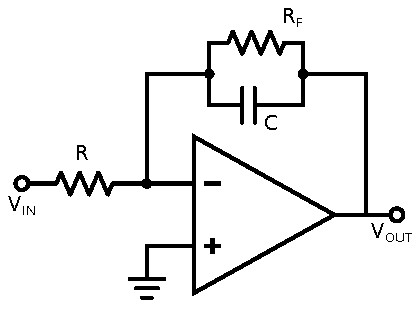
\includegraphics[width=55mm]{ccint.pdf}
	\label{fig:ccsum}
\end{wrapfigure}

\section{Integratore}

In questa parte dell'esperienza utilizzeremo un cazzo di op-amp per costruire un circuito integratore. Lo schema è riportato in Fig.(\ref{}). Analizziamolo assumendo che $R_f=\infty$\footnote{Senza tale approssimazione risulta particolarmente complicata la trattazione del circuito.}. È semplice ricavare $I=C\frac{d(V_A-V_{out})}{dt}$ da cui $V_{in}=-RC\frac{V_{out}}{dt}$. Non siamo matematici ma la seguente relazione è triviale:

$$V_{out}=-\frac{1}{RC} \int V_{in}dt +costante$$

I valori di resistenze e capacità utilizzate sono $R=(99.2 \pm 0.1)\si{\kilo\ohm}$, $R_f=(2.247 \pm 0.001)\si{\mega\ohm}$ e $C=(0.097 \pm 0.002) \si{\micro\farad}$. 

Poiche il condensatore, come sappiamo, taglia i segnali continui, dobbiamo preoccuparci di calcolare la frequenza di taglio. Assumendo trascurabile il contributo dato da $R_f$ e dalla resistenza interna dell'oscilloscopio (entrambe molto grandi, dell'ordine del $\si{\mega\ohm}$), la frequenza di taglio approssimativamente è stimabile da $f\simeq \frac{1}{2\pi C R_1}$. Inserendo i valori numerici otteniamo $f \simeq 15 \si{\hertz}$. Abbiamo dunque deciso di utilizzare dei segnali in ingresso a frequenza di \SI{10}{\hertz}. Abbiamo tuttavia provato anche per frequenze di \SI{1}{\kilo\hertz}. I risultati sono esposti nei seguenti grafici.